\loesung{
\begin{enumerate}[a)]
  \item Calculation of Pearson correlation coefficient of $x_1$ and $x_2$
  $$
 \rho(x_1, x_2) = \frac{\sum_{i = 1}^n (x_1^{(i)} - \overline{x}_1)(x_2^{(i)} - \overline{x}_2)}{\sqrt{\sum_{i = 1}^n (x_1^{(i)} - \overline{x}_1)^2} \sqrt{\sum_{i = 1}^n (x_2^{(i)} - \overline{x}_2)^2}}
  $$ 
   
  given the dataset

 \begin{table}[ht]
\centering
\begin{tabular}{rrrrrrrrrr|r}
\hline
& 1 & 2 & 3 & 4 & 5 & 6 & 7 & 8 & 9 & $\sum_{i = 1}^n$ \\ 
\hline
y & -7.79 & -5.37 & -4.08 & -1.97 & 0.02 & 2.05 & 1.93 & 2.16 & 2.13 & -10.92\\ 
$x_1$ & -1.00 & -0.75 & -0.50 & -0.25 & 0.00 & 0.25 & 0.50 & 0.75 & 1.00 & 0 \\ 
$x_2$ & 0.95 & 0.57 & 0.29 & -0.03 & 0.02 & 0.08 & 0.23 & 0.54 & 0.98 & 3.63 \\ 
\hline
\end{tabular}
\end{table}
 
The individual differences to the means are
 
\begin{table}[H]
\centering
\begin{tabular}{rrrrrrrrrr}
  \hline
 & 1 & 2 & 3 & 4 & 5 & 6 & 7 & 8 & 9  \\ 
\hline
  $x_1^{(i)} - \overline{x}_1$ & -1.00 & -0.75 & -0.50 & -0.25 & 0.00 & 0.25 & 0.50 & 0.75 & 1.00 \\ 
  $x_2^{(i)} - \overline{x}_2$ & 0.55 & 0.17 & -0.11 & -0.43 & -0.38 & -0.32 & -0.17 & 0.14 & 0.58 \\ 
   \hline
\end{tabular}
\end{table}
  
     $$ 
    \begin{aligned}
  \rho(x_1, x_2) & = \frac{\sum_{i = 1}^n (x_1^{(i)} - \overline{x}_1)(x_2^{(i)} - \overline{x}_2)}{\sqrt{\sum_{i = 1}^n (x_1^{(i)} - \overline{x}_1)^2} \sqrt{\sum_{i = 1}^n (x_2^{(i)} - \overline{x}_2)^2}} \\
  & = \frac{-0.574 + -0.125 + 0.057 + 0.108 + 0 + -0.081 + -0.087 + 0.103 + 0.577}{2.086} = \frac{0.05}{2.086} = 0.002
    \end{aligned}
  $$ 
  
  The Pearson correlation coefficient is close to 0 $\Rightarrow$ there is \textbf{no linear} relationship between $x_1$ and $x_2$.
  
  \item  The scatter plot reveals that there is a strong non-linear/quadratic relationship between $x_1$ and $x_2$. The Pearson correlation coefficients is not suitable for detecting non-linear relationships.
  
	\begin{center}
	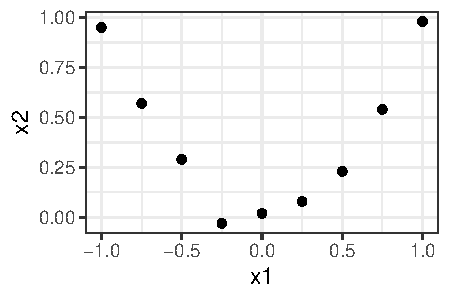
\includegraphics[width=\maxwidth]{figure/add_Points_x1_x2_sol.pdf}
	\end{center}

  \item[$\Rightarrow$] More suitable: \textbf{Mutual Information (MI)}
  
  \begin{align*}
  	MI(x_1 ; x_2 ) =  \mathbb{E}_{p(x_1, x_2)} \left[ log\left(\frac{p(x_1, x_2)}{p(x_1) p(x_2)} \right) \right] = \sum_{x_1} \sum_{x_2} p(x_1, x_2) log\left(\frac{p(x_1, x_2)}{p(x_1) p(x_2)} \right)
  \end{align*}
  Problem: distribution needed. \\
  Solution: e.g. histograms with Gaussian kernel:
  \begin{center}
  	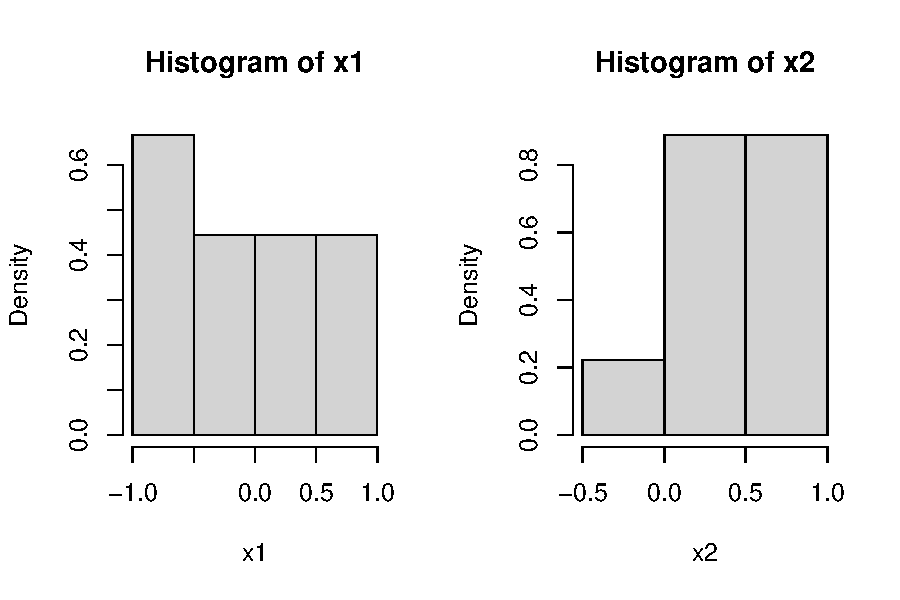
\includegraphics[width=0.8\maxwidth]{figure/hist_x1_x2.pdf}
  \end{center}
  Now taking the mean values as replacement for the values in $x_1$ and $x_2$:
  \begin{table}[H]
  	\centering
  	\begin{tabular}{r|rrrrrrrrr}
  		\hline
  		& 1 & 2 & 3 & 4 & 5 & 6 & 7 & 8 & 9 \\ 
  		\hline
  		$x_1^\star$ & -0.75 & -0.75 & -0.75 & -0.25 & -0.25 & 0.25 & 0.25 & 0.75 & 0.75 \\ 
  		$x_2^\star$ & 0.75 & 0.75 & 0.25 & -0.25 & 0.25 & 0.25 & 0.25 & 0.75 & 0.75 \\ 
  		\hline
  	\end{tabular}
  \end{table}  
  Table with joint and marginal distribution: 
  \begin{table}[H]
  	\centering
  	\begin{tabular}{r|rrr|r}
  		\hline
  		$x_1^\star$ / $x_2^\star$& -0.25 & 0.25 & 0.75 & $p_{x_1}$ \\ 
  		\hline
  		-0.75 & 0.00 & 0.11 & 0.22 & 0.33 \\ 
  		-0.25 & 0.11 & 0.11 & 0.00 & 0.22 \\ 
  		0.25 & 0.00 & 0.22 & 0.00 & 0.22 \\ 
  		0.75 & 0.00 & 0.00 & 0.22 & 0.22 \\
  		\hline 
  		$p_{x_2}$& 0.11 & 0.44 & 0.44 & 1.00 \\ 
  		\hline
  	\end{tabular}
  \end{table}
Now we can calculate the approximate MI: 
   \begin{align*}
   	MI(x_1^\star ; x_2^\star) = & \sum_{x_1^\star} \sum_{x_2^\star} p(x_1^\star, x_2^\star) \, log\left(\frac{p(x_1^\star, x_2^\star)}{p(x_1^\star) p(x_2^\star)} \right)\\
 	=& \,0\, log\left(\frac{0}{0.33 \cdot 0.11} \right) 
   	+ 0.11\, log\left(\frac{0.11}{0.33 \cdot 0.44} \right) 
   	+ 0.22\, log\left(\frac{0.22}{0.33 \cdot 0.44} \right) \\
   	&+ 0.11\, log\left(\frac{0.11}{0.22 \cdot 0.11} \right)
   	+ 0.11\, log\left(\frac{0.11}{0.22 \cdot 0.44} \right) 
   	+ 0\, log\left(\frac{0}{0.22 \cdot 0.44} \right) \\
   	&+ 0\, log\left(\frac{0}{0.22 \cdot 0.11} \right)
   	+ 0.22\, log\left(\frac{0.22}{0.22 \cdot 0.44} \right) 
   	+ 0\, log\left(\frac{0}{0.22 \cdot 0.44} \right) \\
   	&+ 0\, log\left(\frac{0}{0.22 \cdot 0.11} \right)
   	+ 0\, log\left(\frac{0}{0.22 \cdot 0.44} \right) 
   	+ 0.22\, log\left(\frac{0.22}{0.22 \cdot 0.44} \right) \\
   	= & \, 0.603
   \end{align*}
$\Rightarrow$ MI shows that there is a dependency.
  
 
%  \item The p-value of $2.79 \times 10^{-5}$ (but also the adjusted $R^2$ value) reveals that there is a strong relationship between $x_1$ and $x_2$.
%  The p-value does not reveal the shape of this relationship.
  
\end{enumerate}
}
